
\begin{lstlisting}[language=Python]
    import pandas as pd
import numpy as np
import matplotlib.pyplot as plt
from tqdm import tqdm
from sklearn.ensemble import AdaBoostClassifier
from sklearn.datasets import make_classification
from sklearn.model_selection import train_test_split
# Cria um problema de classificacao artificial
X, y = make_classification(n_samples=2000, n_features=10,
            n_informative=8, n_redundant=0,
            random_state=0, shuffle=False)
# Separa dados em treino e teste
X_train, X_test, y_train, y_test = train_test_split(
            X, y, test_size=0.3, random_state=0)

train_errors = []
test_errors = []
interval = np.arange(1, 250, 10)

for i in tqdm(interval):
    clf = AdaBoostClassifier(n_estimators=i, random_state=0)
    clf.fit(X_train, y_train)
    train_errors.append(1 - clf.score(X_train, y_train))
    test_errors.append(1 - clf.score(X_test, y_test))




plt.plot(interval, train_errors, label="train")
plt.plot(interval, test_errors, label="test")
plt.legend()



\end{lstlisting}

\begin{figure}[H]
    \centering
    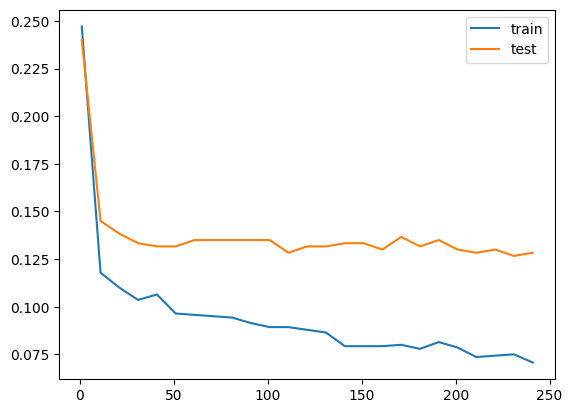
\includegraphics[width=0.8\textwidth]{../figures/2/output.png}
    \caption{Curva de erro de treinamento e teste a cada iteração}
\end{figure}

A figura acima demonstra a evolução do erro de treinamento e teste a cada iteração
do AdaBoost. O erro de treinamento diminui continuamente, apesar de demonstrar
pequenos aumentos em alguns pontos, o que é esperado dado o processo de reamostragem. Já o
erro de teste inicialmente diminui, atingindo um plateau, que se mantem até o final
do processo. Ao contrário do Random Forest ou Bagging, o AdaBoost pode
apresentar overfitting, de modo que, caso aumentemos o número de iterações, é
possível que o erro de teste comece a aumentar, enquanto o erro de treinamento
continuará a diminuir.
